\section{\textit{A Priori} Analysis}
\label{sec:subfilter:dns}

\subsection{DNS Database}
\label{sec:subfilter:dns:database}

The effectiveness of the proposed $Z$-activated soot subfilter PDF at reducing the oxidation rate is validated through an \textit{a priori} analysis using the database from a three-dimensional DNS of a temporally evolving, turbulent nonpremixed planar jet flame at atmospheric pressure~\cite{attili2014}. In this simulation, a central fuel slab consisting of an \textit{n}-heptane/nitrogen [15/85 by volume] mixture at 400 K is surrounded on either side by an air coflow at 800 K. The initial velocity field of the fuel jet is obtained from an instantaneous realization of a turbulent channel flow at $Re_{\tau} = 390$ with a centerline value of $U_c = 8.74$ m/s. The surrounding air flows in the opposite direction of the fuel jet with a streamwise velocity of the same magnitude to give a jet Reynolds number $Re = 2U_c H/\nu \approx 15,000$.

Oxidation of \textit{n}-heptane is modeled with a reduced mechanism comprising 47 species and 290 reactions that accounts for the formation of PAH up to naphthalene. The soot model, as described in \cref{ch:lesmodels,ch:subfilter}, is used in both the DNS and the \textit{a priori} analysis. In the DNS, the soot population is described with seven statistical moments whereas only three moments and the weight of the delta function are used in the \textit{a priori} investigation. The choice to use a reduced set of moments allows for validation of the proposed soot model in a configuration that will most likely be implemented in LES.

The DNS domain is discretized with $N_x \times N_y \times N_z = 1024 \times 1024 \times 512$ grid points, where the homogeneous region of the domain ($|y/H| \le 2.8$) has a grid spacing of $h = 91\ \mu$m. For a filter width $\Delta$, the \textit{a priori} study utilizes a subset of the domain of size $N_x \times N_y \times (\Delta/h + 1)$, where low-pass filtering is done only within the homogeneous mesh region. Additionally, analysis is performed on a snapshot of the DNS at $t = 5$ ms and at a stoichiometric scalar dissipation rate of $\chi_{st} = 20$ s$^{-1}$. Other key properties of the DNS are summarized in \cref{tab:subfilter:dns:params}, and complete details can be found in Attili et al.~\cite{attili2014}.

\begin{table}[htbp]
\centering
\caption[Parameters for DNS of Turbulent Nonpremixed \ce{C7H16}/\ce{N2} Jet Flame]{Parameters for DNS of a turbulent nonpremixed \ce{C7H16}/\ce{N2} jet flame}
\label{tab:subfilter:dns:params}
\begin{tabular}{p{0.46\textwidth} p{0.15\textwidth} p{0.2\textwidth}}
\toprule
Initial jet width, $H$
& [mm] & 15 \\[0.2em]

Domain size, $L_x \times L_y \times L_z$
& [mm] & $94 \times 105 \times 47$ \\[0.2em]

Time step, $\Delta t$
& [$\mu$s] & 4 \\[0.2em]

Minimum Kolmogorov scale, $\eta$
& [$\mu$m] & 110 \\[0.2em]

Kinematic viscosity of fuel mixture, $\nu$
& [m$^2$s$^{-1}$] & $1.7 \times 10^{-5}$ \\[0.2em]

Stoichiometric mixture fraction, $Z_{st}$
& [--] & 0.147 \\

\bottomrule
\end{tabular}
\end{table}

In order to validate the proposed LES model against DNS, a low-pass filter must be applied to the chosen snapshot of the DNS database. A three-dimensional, clipped and renormalized Gaussian filter kernel is employed and is given by
\begin{equation}\label{eq:subfilter:dns:kernel}
  F(x,y,z) = \kappa^3\exp\left[ \frac{-6(x^2 + y^2 + z^2)}{\Delta^2} \right],
\end{equation}
where $\Delta$ is the filter width and $\kappa$ is a renormalization constant that ensures the following relation holds for a grid spacing $h$:
\begin{equation}\label{eq:subfilter:dns:unity}
  \sum\limits_{x = -\Delta/2h}^{\Delta/2h} \sum\limits_{y = -\Delta/2h}^{\Delta/2h} \sum\limits_{z = -\Delta/2h}^{\Delta/2h} F(x,y,z) = 1.
\end{equation}
Note that the above relations require a homogeneous mesh such that $\kappa = \kappa_j$, $\Delta = \Delta_j$, and $h = h_j$, where the index $j \in \{ x,y,z \}$. As evident in \cref{eq:subfilter:dns:unity}, the filter kernel is active over a cube of $(\Delta/h + 1)^3$ grid points.


\subsection{Oxidation Source Term}
\label{sec:subfilter:dns:ox}

The filtered moment source term for oxidation is evaluated with the soot subfilter PDFs of \cref{eq:subfilter:leszussp:ox,eq:subfilter:zassp:ox}. The goal of the proposed model is to increase the overall amount of soot, so this analysis will focus on the oxidation source term contribution to the total volume fraction, $\fst[M]{1,0}^{ox}$. Oxidation of only the outermost surface is considered to reduce modeling complexity and computational cost, so the expression for the source term depends on the filtered moment for the total soot surface area $\mean{M}_{0,1}$.

Several approximations need to be made with regards to \cref{eq:subfilter:zassp:ox} before the \textit{a priori} analysis can be performed. First, the oxidation coefficient $k_{ox}(Z)$ is not present in the DNS database, as it was originally obtained from a flamelet model. However, spatial fields of density and mixture fraction are available, and the oxidation coefficient can be calculated as a function of space. Thus, $k_{ox}(Z)$ will be estimated with a density-weighted conditional average
\begin{equation}\label{eq:subfilter:dns:condkox}
  \begin{split}
    k_{ox}(Z) &\approx \{ k_{ox}(x_j)|Z(x_j) \} \\
    &= \frac{<\rho(x_j)k_{ox}(x_j)|Z(x_j)>}{<\rho(x_j)|Z(x_j)>},
  \end{split}
\end{equation}
where the angle brackets $< \cdot >$ denote the conditional averaging operator and the curly brackets $\{ \cdot \}$ denote the density-weighted conditional averaging operator. This quantity is plotted in \cref{fig:subfilter:dns:kox}, where it is evident that the oxidation coefficient at mixture fractions $Z < 0.1$ and $Z > 0.4$ is well-approximated by \cref{eq:subfilter:dns:condkox}. However, the large spread of the DNS field in $0.1 < Z < 0.4$ indicates that additional conditional averaging against the scalar dissipation rate or another variable could be performed for a more accurate approximation.

\begin{figure}[htb]
  \centering
  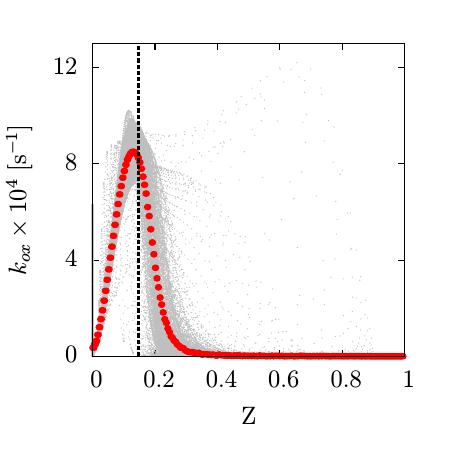
\includegraphics[width=0.4\linewidth]{ch-subfiltermodeling/figures/koxvsz}
  \caption[Approximation for Oxidation Coefficient, \texorpdfstring{$k_{ox}(Z)$}{kox(Z)}]{Density-weighted, conditionally averaged approximation for the oxidation coefficient $k_{ox}(Z)$. The gray dots represent $k_{ox}(x_j)|Z(x_j)$ from DNS and the red circles are the approximation $\{ k_{ox}(x_j)|Z(x_j) \}$, evaluated with 200 bins. The vertical black dashed line marks the location of stoichiometric mixture fraction $Z_{st} = 0.147$.}
  \label{fig:subfilter:dns:kox}
\end{figure}

The second quantity that needs to be estimated is the thermochemical subfilter PDF $\pz$, since the DNS database does not have the infinite number of points required to construct the true subfilter distribution. As before, this work will presume the form of a beta PDF for $\pz$. The error associated with this assumption can be discerned by juxtaposing two versions of \cref{eq:subfilter:leszussp:ox} that use the same $Z$-uniform soot subfilter PDF but approximate $k_{ox}(Z)$ with and without $\pz$. The form of the filtered moment source term for oxidation that excludes $\pz$ shall be referred to as the ``ZUSSP without $\pz$'' case and is given by
\begin{equation}\label{eq:subfilter:dns:mzusspwithoutpz}
  \fst[M]{1,0}^{ox} = \{ \tf{k_{ox}(x_j)|Z(x_j)} \} \cdot \mean{M_{0,1}(x_j)},
\end{equation}
where the $\tf{(\cdot)}$ operator denotes the density-weighted version of the low-pass filtering operator $\mean{(\cdot)}$. Use of the $Z$-uniform soot subfilter PDF implies that the soot scalars are assumed to be independent of the thermochemical variables. This property is evident in \cref{eq:subfilter:dns:mzusspwithoutpz}, where the two components are distinctly separated.

The source term using $\pz$ will be referred to as the ``ZUSSP with $\pz$'' case, and is given by
\begin{equation}\label{eq:subfilter:dns:mzusspwithpz}
  \fst[M]{1,0}^{ox} = \int\limits_0^1 \{ k_{ox}|Z \}\pz dZ \cdot \mean{M_{0,1}(x_j)},
\end{equation}
where $\{ k_{ox}|Z \}$ is the density-weighted, conditionally averaged oxidation coefficient that is not a function of space. \cref{eq:subfilter:dns:mzusspwithoutpz,eq:subfilter:dns:mzusspwithpz} are first individually compared to the filtered moment source term from DNS, which will be referred to as the ``DNS'' case and is given by
\begin{equation}\label{eq:subfilter:dns:mdns}
  \fst[M]{1,0}^{ox} = \mean{\{ k_{ox}(x_j)|Z(x_j)\} \cdot M_{0,1}(x_j)}.
\end{equation}
These comparisons are visible for a filter width of $\Delta/h = 32$ in \cref{fig:subfilter:dns:erroronbetaox}. The top two plots show that \cref{eq:subfilter:dns:mzusspwithoutpz,eq:subfilter:dns:mzusspwithpz} generally overpredict the oxidation rate compared to the value from DNS. However, when they are compared with each other in the bottom left plot, the sample standard deviation is roughly an order of magnitude smaller. This suggests that the error associated with presuming the form of a beta distribution for $\pz$ is less than the error associated with using the $Z$-uniform soot subfilter PDF to evaluate the filtered moment source term for oxidation.

The validity of presuming the beta distribution is more easily elucidated in the bottom right plot of \cref{fig:subfilter:dns:erroronbetaox}, where the cumulative distribution function (CDF) is plotted for $\fst[M]{1,0}^{ox}$. It can be observed that the distance between the lines representing \cref{eq:subfilter:dns:mzusspwithoutpz,eq:subfilter:dns:mzusspwithpz} is generally much less than the deviation between the latter and the source term from DNS. However, this trend is not valid when the magnitude of the source term is on the order of $10^2$ to $10^3$, where the error of presuming a beta distribution is commensurate with the error from the form of the soot subfilter PDF. Nevertheless, the most important values of the source term are the largest, where the error associated with presuming the form of a beta distribution for $\pz$ is relatively small.  This trend holds true for larger filter widths as well.

\begin{figure}[ht]
  \centering
  \begin{subfigure}[b]{0.375\linewidth}
    \centering
    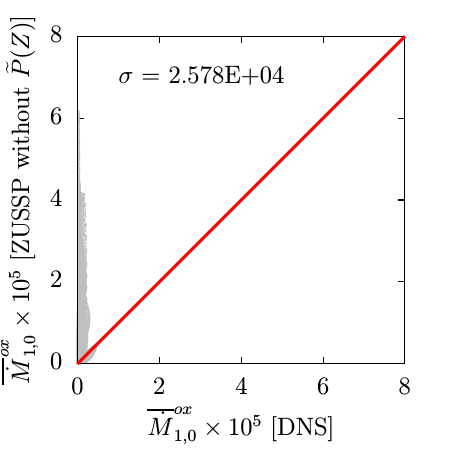
\includegraphics[width=\linewidth]{ch-subfiltermodeling/figures/lin-Mox3vsMox6-r3D-32}
    %\vspace{1ex}
  \end{subfigure}%%
  \begin{subfigure}[b]{0.375\linewidth}
    \centering
    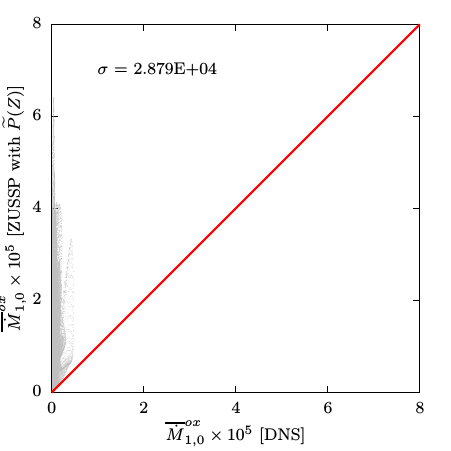
\includegraphics[width=\linewidth]{ch-subfiltermodeling/figures/lin-Mox4vsMox6-r3D-32}
    %\vspace{1ex}
  \end{subfigure}
  \begin{subfigure}[b]{0.375\linewidth}
    \centering
    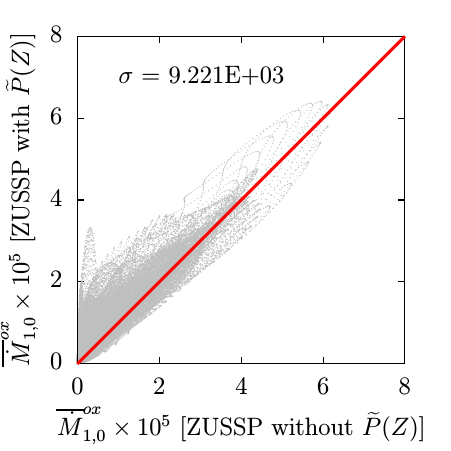
\includegraphics[width=\linewidth]{ch-subfiltermodeling/figures/lin-Mox4vsMox3-r3D-32}
  \end{subfigure}%%
  \begin{subfigure}[b]{0.375\linewidth}
    \centering
    \includegraphics[width=\linewidth]{ch-subfiltermodeling/figures/cdf-ox-ZUSSP-r3D-32}
  \end{subfigure}
  \caption[Error Associated with \texorpdfstring{$\pz = \beta(Z;\tf{Z},\tf{Z_V})$}{P(Z) = B(Z;Z,ZV)} for \texorpdfstring{$\fst[M]{1,0}^{ox}$}{M1,0ox}]{Filtered moment source term for oxidation at $t = 5$ ms evaluated with \cref{eq:subfilter:dns:mzusspwithoutpz,eq:subfilter:dns:mzusspwithpz,eq:subfilter:dns:mdns} for a filter width of $\Delta/h = 32$. In the first three plots, the red lines represent a one-to-one correspondence and the sample standard deviation is indicated at the top left corner. In the fourth, bottom right plot, the solid red line is the ``DNS'' case, the blue dashed line is the ``ZUSSP without $\pz$'' case, and the blue dash-dotted line is the ``ZUSSP with $\pz$'' case.}
  \label{fig:subfilter:dns:erroronbetaox}
\end{figure}

Now that the form of the thermochemical subfilter PDF $\pz$ has been confirmed, the filtered moment source term for oxidation using the $Z$-activated soot subfilter PDF can be evaluated. The latter shall be referred to as the ``ZASSP with $\pz$'' case and its expression is given by
\begin{equation}\label{eq:subfilter:dns:mzasspwithpz}
  \fst[M]{1,0}^{ox} = \frac{\int\limits_0^1 \{ k_{ox}|Z \}H(Z - Z_{st})\pz dZ}{\int\limits_0^1 H(Z - Z_{st})\pz dZ} \cdot \mean{M_{0,1}(x_j)}.
\end{equation}

This case is plotted against the source term from DNS in \cref{fig:subfilter:dns:zasspcomparison}. In the left-hand plot, it is clear that the filtered moment source term for oxidation evaluated with the proposed model still overpredicts the oxidation rate when compared to the values from DNS. However, when contrasted with the top right plot of \cref{fig:subfilter:dns:erroronbetaox}, the magnitudes of the largest source terms are reduced by nearly half and the standard deviation is decreased. A direct comparison between the source terms using the $Z$-uniform and $Z$-activated soot subfilter PDFs, available in the middle plot of \cref{fig:subfilter:dns:zasspcomparison}, demonstrates that the latter tends to produce smaller oxidation rates than the former. This is to be expected, as the $Z$-activated soot subfilter PDF was formulated to eliminate the unphysical contributions to the oxidation rate that the $Z$-uniform soot subfilter PDF possessed.

The CDF in the right-hand plot of \cref{fig:subfilter:dns:zasspcomparison} more clearly reveals the extent of the oxidation source term reduction. It is evident that the proposed model has decreased the largest values of the source term relative to the ``ZUSSP with $\pz$'' case, albeit the effect is not enough to reach the values of the source terms from DNS. Nevertheless, the effectiveness of the proposed model is expected to increase with the filter width due to the expanded presence of lean subfilter regions, which is a consequence of the enlargened variance in mixture fraction. This point will be explored in \cref{sec:subfilter:dns:fw}.

\begin{figure}[ht]
  \centering
  \begin{subfigure}[b]{0.33\linewidth}
    \centering
    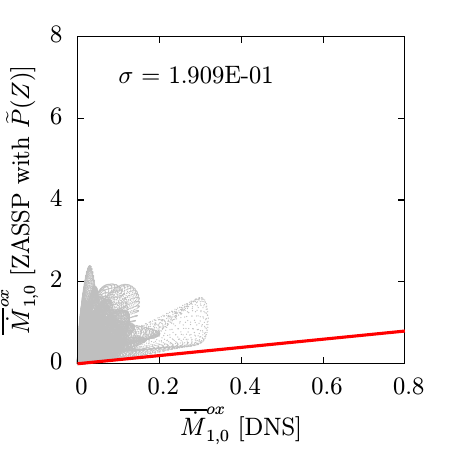
\includegraphics[width=\linewidth]{ch-subfiltermodeling/figures/lin-Mox5vsMox6-r3D-32}
  \end{subfigure}%%
  \begin{subfigure}[b]{0.33\linewidth}
    \centering
    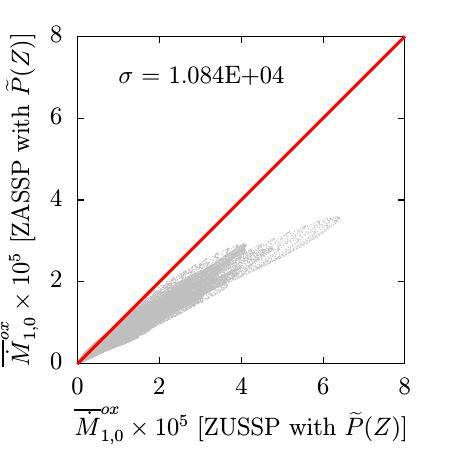
\includegraphics[width=\linewidth]{ch-subfiltermodeling/figures/lin-Mox5vsMox4-r3D-32}
  \end{subfigure}%%
  \begin{subfigure}[b]{0.33\linewidth}
    \centering
    \includegraphics[width=\linewidth]{ch-subfiltermodeling/figures/cdf-ox-ZASSP-r3D-32}
  \end{subfigure}
  \caption[Comparison of ZASSP with $\pz$ to DNS \& ZUSSP with $\pz$ for \texorpdfstring{$\fst[M]{1,0}^{ox}$}{M1,0ox}]{Comparison of the ``ZASSP with $\pz$'' case to the ``DNS'' and ``ZUSSP with $\pz$'' cases for the same conditions as in \cref{fig:subfilter:dns:erroronbetaox}. In the right-hand plot, the solid red line is the ``DNS'' case, the blue dash-dotted line is the ``ZUSSP with $\pz$'' case, and the magenta dash-dotted line is the ``ZASSP with $\pz$'' case.}
  \label{fig:subfilter:dns:zasspcomparison}
\end{figure}


\subsection{Surface Growth Source Term}
\label{sec:subfilter:dns:sg}

Analysis of surface growth source term.


\subsection{Effects of Filter Width}
\label{sec:subfilter:dns:fw}

Investigation of filter width variation effects.


